\section{Heaviside and the Notation of Modern Motion}

\subsection{The Notation Revolution}

By the late 19th century, the ideas of Lagrange and Riemann had given us a new vision of physics — one governed by structure, optimization, and local geometry.  
But there was still a problem: the notation was a mess.

Equations sprawled across pages. Dot products were embedded in prose. Gradients were implied rather than written. Mathematicians understood what they were doing — but no one else did.

Then came \textbf{Oliver Heaviside}.

Heaviside wasn’t interested in inventing new laws — he wanted to clarify the ones we already had.

His contribution was shockingly simple:  \textbf{Clean up the language. Simplify the symbols. Let the structure speak.}

He introduced:

\begin{itemize}
    \item The modern gradient (\( \nabla f \)), divergence (\( \nabla \cdot \vec{F} \)), and curl (\( \nabla \times \vec{F} \)) operators
    \item The dot product (\( \vec{a} \cdot \vec{b} \)) as a compact projection
    \item The idea that physical laws could be written as **local differential operators**
\end{itemize}

He translated the sprawling, coordinate-heavy expressions of 19th-century physics into something modular, symbolic, and — most importantly — readable.

\subsection{A New Way to Write Change}

Heaviside’s notation didn’t just clean things up — it revealed deeper structure.

When we write:
\[
\text{grad}_g f = \nabla_g f
\]
we’re no longer just describing change — we’re encoding geometry. The symbol \( \nabla \) now carries the context of the space it lives in: flat, curved, stretched, or twisted.

This shift from equations to **operators** was transformative.

\subsection{Kepler’s Second Law, Written Cleanly}

Let’s return, one last time, to our running example.

We know:
\begin{itemize}
  \item The planet moves through a gravitational potential \( f = V(q_1) \)
  \item The geometry of space is described by a Riemannian metric \( g \)
  \item The motion respects angular momentum — and thus, Kepler’s Second Law
\end{itemize}

In modern notation, we can now describe this with:
\[
\vec{v}(t) = -\nabla_g f
\quad \text{with} \quad
\frac{dA}{dt} = \text{const}
\]

The first equation tells us how motion flows: along the negative gradient, but weighted by geometry.  
The second encodes the constraint: a conserved geometric quantity, preserved through time.

In Heaviside’s notation, the full system — gravity, geometry, motion — becomes a collection of clean symbolic relationships:
\begin{itemize}
    \item Gradients show direction.
    \item Dot products express alignment.
    \item Time derivatives encode evolution.
\end{itemize}

What had once been written in paragraphs is now a single line.  
Kepler’s Law is no longer a diagram. It’s a differential constraint.

\begin{tcolorbox}[colback=blue!5!white, colframe=blue!50!black, title={Heaviside’s Gift to Kepler}]
Kepler gave us ellipses.  
Lagrange gave us equations.  
Riemann gave us geometry.  
Heaviside gave us clarity.

And with that clarity, we can now write the law of planetary motion —  
not as a story, but as a system.
\end{tcolorbox}

\subsection{Notation as Revelation}

In the end, Heaviside didn’t merely simplify physics —  
he rewired how physicists thought.

Before him, the language of motion and field theory was tangled in verbose prose and component-heavy expressions. Forces were described in coordinates. Potentials were buried in integrals. Gradients, curls, and divergences were known—but not seen.

Then came the operator:
\[
\nabla = \left( \frac{\partial}{\partial x}, \frac{\partial}{\partial y}, \frac{\partial}{\partial z} \right)
\]

With a single symbol, Heaviside made visible what had always been implicit.

\bigskip

\textbf{The gradient} \( \nabla f \) revealed that scalar fields like temperature or potential aren’t just distributions — they have slope, direction, and magnitude at every point. It made it impossible not to see that:
\begin{itemize}
    \item A hill isn’t just high — it points upward.
    \item A potential doesn’t just vary — it flows.
    \item Change isn’t just a value — it’s a vector.
\end{itemize}

\textbf{The divergence} \( \nabla \cdot \vec{F} \) made source strength tangible. Whether modeling electric charge density or compressible fluids, the operator pointed directly to where things emerge, vanish, or compress:
\[
\nabla \cdot \vec{E} = \frac{\rho}{\varepsilon_0}
\]

Suddenly, Gauss’s law wasn’t an abstract integral — it was a differential statement about local behavior.

\textbf{The curl} \( \nabla \times \vec{F} \) made circulation visible. The moment you write:
\[
\nabla \times \vec{v}
\]
you’ve committed to seeing rotation not as a visual aid but as a formal object — a vector that encodes swirling motion.

\bigskip

\begin{quote}
    Gradients are geometry-aware.  
    Divergence exposes creation and collapse.  
    Curl encodes rotation at a point.
\end{quote}

\bigskip

Heaviside’s notation didn’t just compress equations.  
It exposed structure.

It made the local nature of laws transparent:
\begin{itemize}
    \item That motion is directional and differential.
    \item That fields have inner skeletons.
    \item That calculus could encode geometry without coordinates.
\end{itemize}

In doing so, Heaviside moved vector calculus from a tool into a form of perception.  
The physical world wasn’t just describable — it was \textbf{legible}.

\begin{tcolorbox}[colback=gray!5!white, colframe=black, title=\textbf{When Notation Becomes Ontology}, fonttitle=\bfseries, arc=1.5mm, boxrule=0.4pt]
\textbf{Old calculus:} Change is measured.  
\textbf{Heaviside’s calculus:} Change has direction, divergence, and spin.  
Once written symbolically, it becomes irreducibly real.
\end{tcolorbox}



\begin{figure}[H]
    \centering
    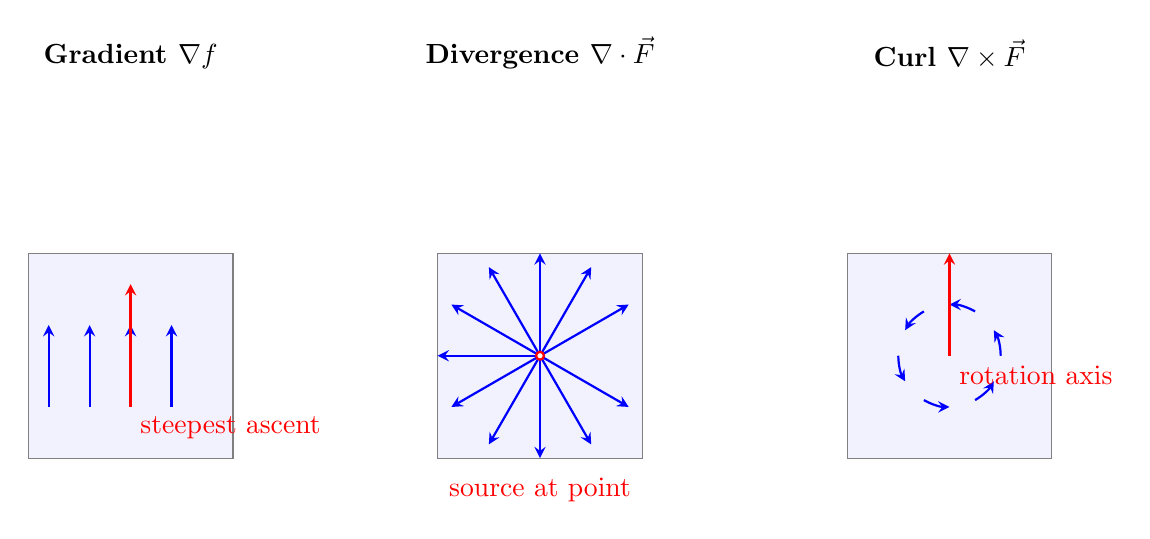
\begin{tikzpicture}[scale=1.3, >=stealth]
    
    % Gradient Panel
    \draw[thick] (-4,1.7) node[anchor=south] {\textbf{Gradient \( \nabla f \)}};
    \draw[fill=blue!5, draw=black!50] (-5,0) rectangle (-3,-2);
    \foreach \x in {-4.8,-4.4,...,-3.2} {
        \draw[->, thick, blue] (\x,-1.5) -- ++(0,0.8);
    }
    \draw[->, thick, red] (-4,-1.5) -- ++(0,1.2);
    \node[red, below right] at (-4,-1.5) {steepest ascent};
    
    % Divergence Panel
    \draw[thick] (0,1.7) node[anchor=south] {\textbf{Divergence \( \nabla \cdot \vec{F} \)}};
    \draw[fill=blue!5, draw=black!50] (-1,0) rectangle (1,-2);
    \foreach \angle in {30,60,...,330} {
        \draw[->, thick, blue] (0,-1) -- ++({cos(\angle)}, {sin(\angle)});
    }
    \draw[red, thick] (0,-1) node[circle, draw=red, inner sep=1pt, fill=white] {};
    
    \node[red, below] at (0,-2.1) {source at point};
    
    % Curl Panel
    \draw[thick] (4,1.7) node[anchor=south] {\textbf{Curl \( \nabla \times \vec{F} \)}};
    \draw[fill=blue!5, draw=black!50] (3,0) rectangle (5,-2);
    \foreach \angle in {0,60,...,300} {
        \draw[->, thick, blue] (4,-1) ++({1*cos(\angle)/2}, {1*sin(\angle)/2}) arc[start angle=\angle, end angle=\angle+30, radius=0.5];
    }
    \draw[->, thick, red] (4,-1) -- ++(0,1);
    \node[red, below right] at (4,-1) {rotation axis};
    
    \end{tikzpicture}
    \caption{Geometric intuition of Heaviside’s operators: the gradient points uphill, divergence reveals local sources, and curl captures rotational structure.}
\end{figure}
    




\subsection{From Heaviside to Exterior Algebra: When Operators Grow Up}

Heaviside’s notation was revolutionary — but it still lived in a very specific world: three-dimensional Euclidean space, with fixed coordinates, cross products, and dot products defined relative to an orthonormal basis.

But what happens when the space isn’t \( \mathbb{R}^3 \)?  
What if you’re on a curved manifold, or you want to express these ideas in four dimensions, or in general relativity?

This is where Heaviside’s operators meet their more mature, abstract cousin:  
\textbf{differential forms and exterior calculus}.

\bigskip

\textbf{Gradient, Divergence, Curl — Reimagined}

In Heaviside’s world:

\[
\nabla f \quad \nabla \cdot \vec{F} \quad \nabla \times \vec{F}
\]

Each operator had a specific mechanical meaning, but they were bound to three-dimensional coordinates and required separate identities and formulas.

In the world of differential forms, everything flows from a single idea:

\[
d: \Omega^k(M) \to \Omega^{k+1}(M)
\]

Where:
\begin{itemize}
    \item \( \Omega^k(M) \) is the space of \( k \)-forms on a manifold \( M \),
    \item \( d \) is the **exterior derivative**, and
    \item \( d^2 = 0 \) encodes the fundamental structure of calculus.
\end{itemize}

\bigskip

\textbf{The dictionary:}
\begin{itemize}
    \item \( \nabla f \) becomes \( df \), a 1-form.
    \item \( \nabla \times \vec{F} \) becomes \( d\omega \), where \( \omega \) is a 1-form representing the vector field.
    \item \( \nabla \cdot \vec{F} \) becomes \( \ast d \ast \omega \), using the Hodge star to express divergence in arbitrary geometry.
\end{itemize}

\bigskip

\textbf{Heaviside:}  
Operators were built by hand.

\textbf{Exterior calculus:}  
Operators emerge naturally from structure.

In this language, Stokes’ theorem doesn’t just describe a special case. It unifies them all:
\[
\int_{\partial \Omega} \omega = \int_\Omega d\omega
\]

This one identity subsumes:
\begin{itemize}
    \item The Fundamental Theorem of Calculus
    \item Green’s Theorem
    \item Gauss’s Divergence Theorem
    \item Stokes’ Theorem (in Heaviside’s vector calculus)
\end{itemize}

\bigskip

\begin{tcolorbox}[colback=gray!5!white, colframe=black, title=\textbf{Sidebar: Vector Calculus vs. Differential Forms}, fonttitle=\bfseries, arc=1.5mm, boxrule=0.4pt]

\textbf{Heaviside:}
\begin{itemize}
  \item Works in \( \mathbb{R}^3 \) only
  \item Gradient, divergence, curl = three separate ideas
  \item Coordinates required
  \item Powerful for electromagnetism and fluids
\end{itemize}

\textbf{Exterior Calculus:}
\begin{itemize}
  \item Works on any manifold
  \item One operator: \( d \)
  \item Coordinate-free and intrinsic
  \item Unifies vector calculus under Stokes’ Theorem
\end{itemize}

\end{tcolorbox}

\bigskip

Heaviside gave us intuition. Exterior calculus gives us invariance.  
One reveals structure. The other ensures it survives transformation.

And when we need to express electromagnetism in curved spacetime,  
we don't use cross products—we reach for forms.

\[
dF = 0 \qquad d \star F = J
\]

Here, in the coordinate-free notation of modern geometry, Maxwell’s equations become elegant and universal.  
No \( \nabla \) in sight — but Heaviside's fingerprints are still all over it.


\begin{tcolorbox}[colback=blue!5!white, colframe=blue!50!black, title={Historical Sidebar: How a Self-Taught Maverick Rewrote Physics Notation}]

    Oliver Heaviside didn’t have a PhD.  He didn’t even have a university degree.

    \medskip
    
    In fact, Heaviside had no formal advanced training at all. He was mostly deaf, socially abrasive, and spent 
    much of his life in isolation — yet he’s the reason modern physicists and engineers write equations the 
    way they do.

    \medskip
    
    A former telegraph operator, Heaviside learned mathematics on his own, driven by frustration with the convoluted 
    formulas used to describe electromagnetic theory. Where academics saw tradition, Heaviside saw inefficiency — 
    and he wasn’t shy about fixing it.

    \medskip
    
    He took James Clerk Maxwell’s sprawling, verbose equations and compressed them into the four elegant expressions 
    we now call \textbf{Maxwell’s Equations}. He introduced the gradient, divergence, and curl symbols. He championed 
    operator notation, making differential equations readable and modular.

    \medskip
    
    The mathematical elite of his time dismissed him as an outsider meddling with things he didn’t "properly" study. 
    Yet today, every physics textbook speaks in Heaviside’s language.
    
    \medskip
    
    \textbf{No degree. No academic post. Just clarity, stubbornness, and a refusal to accept bad notation.}
    \medskip
    
    So next time you effortlessly write \( \nabla \cdot \vec{E} = \frac{\rho}{\varepsilon_0} \), remember — you’re 
    using the tools crafted by a man who never sat through a single formal lecture on vector calculus.

    \medskip
    
    Sometimes, the sharpest revolutions come from people who never learned the rules they’re about to break.
    
\end{tcolorbox}

\subsection*{Reinterpreting Kepler’s Second Law Through Heaviside and Exterior Calculus}

By now, Kepler’s Second Law has worn many robes:  
a geometric sweep, a dynamical symmetry, a surface constraint, a frequency conservation, a geodesic expression.

But in Heaviside’s hands — and in the hands of the modern notation he inspired —  
it becomes something else entirely:

\begin{quote}
A clean differential statement about symmetry, expressed in operators.
\end{quote}

\bigskip

\paragraph{In Heaviside’s Notation.}

We know a planet’s position vector \( \vec{r}(t) \) and velocity \( \vec{v}(t) = \frac{d\vec{r}}{dt} \).  
The areal velocity — the rate at which area is swept out — is given by:

\[
\frac{dA}{dt} = \frac{1}{2} \left\| \vec{r} \times \vec{v} \right\|
\]

Kepler’s Second Law simply says this quantity is conserved.  
In modern operator terms:

\[
\frac{d}{dt} \left( \vec{r} \times \frac{d\vec{r}}{dt} \right) = 0
\]

This expression is short, symbolic, and evocative:  
conservation is written as the vanishing of a time derivative.

\bigskip

\paragraph{In Exterior Calculus.}

Now suppose we step beyond 3D space and ask:  
Can we write this geometrically, without relying on coordinates or cross products?

Yes — via differential forms.

Define the **areal 2-form** on the configuration manifold \( M \) as:

\[
\omega = \frac{1}{2} (\vec{r} \wedge d\vec{r})
\]

Then Kepler’s Second Law becomes:

\[
\mathcal{L}_{\vec{v}} \omega = 0
\]

Where:
\begin{itemize}
  \item \( \omega \) is the area form swept out in the tangent space,
  \item \( \vec{v} \) is the velocity vector field,
  \item \( \mathcal{L}_{\vec{v}} \) is the Lie derivative — the rate of change of \( \omega \) along the motion.
\end{itemize}

This means: \textbf{area is preserved along the flow}.  
Kepler’s law is a differential invariance — a geometric symmetry, written cleanly.

\bigskip

\paragraph{From Notation to Ontology.}

In Heaviside’s vector calculus, the law of areas became a conserved cross product.  
In differential geometry, it becomes the invariance of a 2-form under flow.  
In both, the content is the same — but the expression is cleaner, clearer, and more universal.

\bigskip

\begin{tcolorbox}[colback=blue!5!white, colframe=blue!50!black, title=\textbf{Heaviside's Take on Kepler}]
Kepler saw a sweep.  
Newton wrote a force.  
Riemann curved the space.  
Heaviside made it readable.  
Exterior calculus made it eternal.
\end{tcolorbox}
